%%%%%%%%%%%%%%%%%%%%%%%%%%%%%%%%%%%%%%%%%
% Beamer Presentation
% LaTeX Template
% Version 1.0 (10/11/12)
%
% This template has been downloaded from:
% http://www.LaTeXTemplates.com
%
% License:
% CC BY-NC-SA 3.0 (http://creativecommons.org/licenses/by-nc-sa/3.0/)
%
%%%%%%%%%%%%%%%%%%%%%%%%%%%%%%%%%%%%%%%%%

%----------------------------------------------------------------------------------------
%	PACKAGES AND THEMES
%----------------------------------------------------------------------------------------

\documentclass[10pt]{beamer}

\mode<presentation> {

% The Beamer class comes with a number of default slide themes
% which change the colors and layouts of slides. Below this is a list
% of all the themes, uncomment each in turn to see what they look like.

\usetheme{default}
% \usetheme{AnnArbor}
% \usetheme{Antibes}
% \usetheme{Bergen}
% \usetheme{Berkeley}
% \usetheme{Berlin}
% \usetheme{Boadilla}
% \usetheme{CambridgeUS}
% \usetheme{Copenhagen}
% \usetheme{Darmstadt}
% \usetheme{Dresden}
% \usetheme{Frankfurt}
% \usetheme{Goettingen}
% \usetheme{Hannover}
% \usetheme{Ilmenau}
% \usetheme{JuanLesPins}
% \usetheme{Luebeck}
% \usetheme{Madrid}
% \usetheme{Malmoe}
% \usetheme{Marburg}
% \usetheme{Montpellier}
% \usetheme{PaloAlto}
% \usetheme{Pittsburgh}
% \usetheme{Rochester}
% \usetheme{Singapore}
% \usetheme{Szeged}
% \usetheme{Warsaw}

% As well as themes, the Beamer class has a number of color themes
% for any slide theme. Uncomment each of these in turn to see how it
% changes the colors of your current slide theme.

% \usecolortheme{albatross}
% \usecolortheme{beaver}
% \usecolortheme{beetle}
% \usecolortheme{crane}
% \usecolortheme{dolphin}
% \usecolortheme{dove}
% \usecolortheme{fly}
% \usecolortheme{lily}
% \usecolortheme{orchid}
% \usecolortheme{rose}
% \usecolortheme{seagull}
\usecolortheme{seahorse}
% \usecolortheme{whale}
% \usecolortheme{wolverine}

%\setbeamertemplate{footline} % To remove the footer line in all slides uncomment this line
\setbeamertemplate{footline}[page number] % To replace the footer line in all slides with a simple slide count uncomment this line

\setbeamertemplate{navigation symbols}{} % To remove the navigation symbols from the bottom of all slides uncomment this line
}

\graphicspath{ {./figures/} }
\usepackage{graphicx} % Allows including images
\usepackage{booktabs} % Allows the use of \toprule, \midrule and \bottomrule in tables

%----------------------------------------------------------------------------------------
%	TITLE PAGE
%----------------------------------------------------------------------------------------

\title[Data Science in Blackwell]{Notes on Expanding Internal Data Mining Efforts} % The short title appears at the bottom of every slide, the full title is only on the title page

\author{Tuomo Kareoja} % Your name
\institute[Blackwell] % Your institution as it will appear on the bottom of every slide, may be shorthand to save space
{
Blackwell \\ % Your institution for the title page
\medskip
}
\date{\today} % Date, can be changed to a custom date

\begin{document}

\begin{frame}
\titlepage % Print the title page as the first slide
\end{frame}

% \begin{frame}
% \frametitle{Overview} % Table of contents slide, comment this block out to remove it
% \tableofcontents % Throughout your presentation, if you choose to use \section{} and \subsection{} commands, these will automatically be printed on this slide as an overview of your presentation
% \end{frame}

%----------------------------------------------------------------------------------------
%	PRESENTATION SLIDES
%----------------------------------------------------------------------------------------

%------------------------------------------------
\section{Newest Data Mining Projects} % Sections can be created in order to organize your presentation into discrete blocks, all sections and subsections are automatically printed in the table of contents as an overview of the talk
%------------------------------------------------

%------------------------------------------------
\subsection{Filling Missing Data with a Predictive Model} % A subsection can be created just before a set of slides with a common theme to further break down your presentation into chunks
%------------------------------------------------

\begin{frame}
\frametitle{Filling Missing Data with a Predictive Model}
% Uncomment the code on this slide to include your own image from the same directory as the template .TeX file.

\begin{columns}[c] % The "c" option specifies centered vertical alignment while the "t" option is used for top vertical alignment

\column{.4\textwidth} % Left column and width

\textbf{Problem:} Some of the customer data has missing values and this could skew further analyses if not fixed

\uncover<2->{
\textbf{Solution:} Create a model to predict the missing values from the values of the other columns
}

\uncover<3->{
\textbf{Knowledge Gained:} The data are missing at random so the missing values don't skew the analysis
}

\column{.6\textwidth} % Right column and width

\uncover<1->{
\begin{figure}
    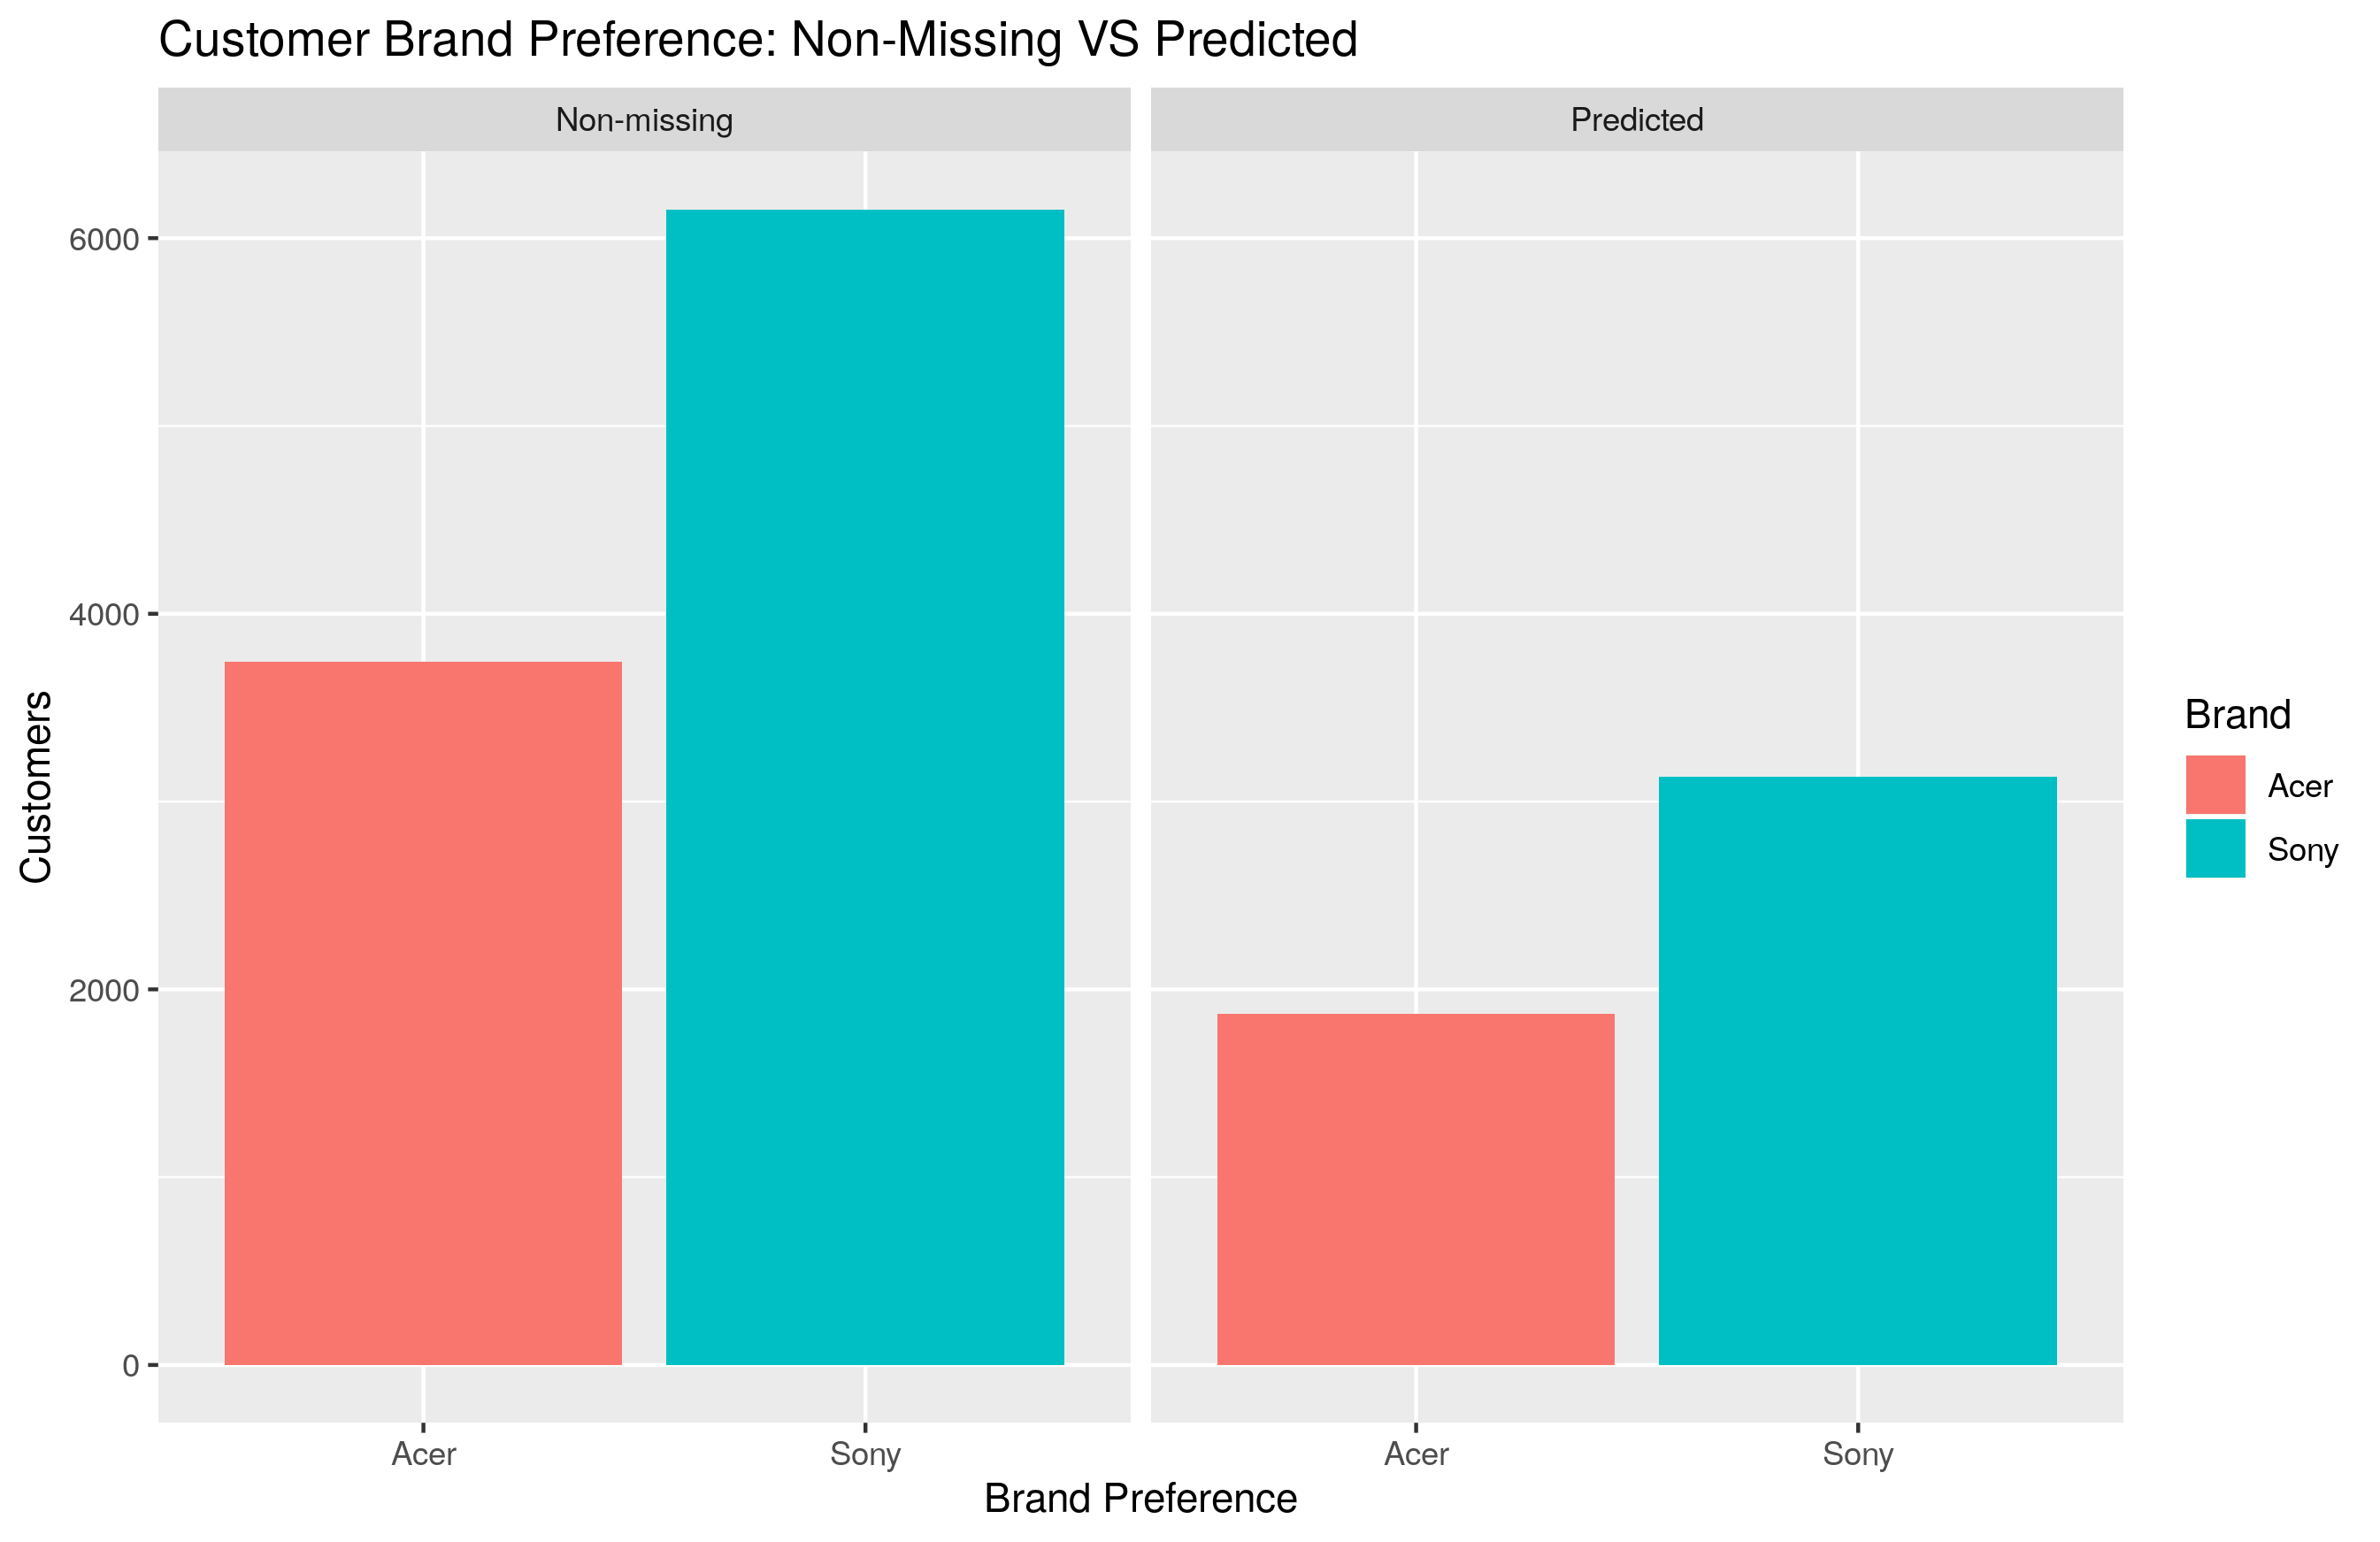
\includegraphics[width=1.1\linewidth, keepaspectratio]{brand_preference_marked.png}
\end{figure}
}

\end{columns}

\end{frame}

%------------------------------------------------
\subsection{Predicting Sales of Upcoming Products} % A subsection can be created just before a set of slides with a common theme to further break down your presentation into chunks
%------------------------------------------------

\begin{frame}
\frametitle{Predicting Sales of Upcoming Products}

\begin{columns}[c] % The "c" option specifies centered vertical alignment while the "t" option is used for top vertical alignment

\column{.4\textwidth} % Left column and width

\textbf{Problem:} We would want to know the future sales volumes of our upcoming products

\uncover<2->{
\textbf{Solution:} Create a model to predict the sales volume from customer reviews and product attributes
}

\uncover<3->{
\textbf{Knowledge Gained:} Some products are predicted to perform way better than others, but a better model
would need more data
}

\column{.6\textwidth} % Right column and width

\uncover<1->{
\begin{figure}
    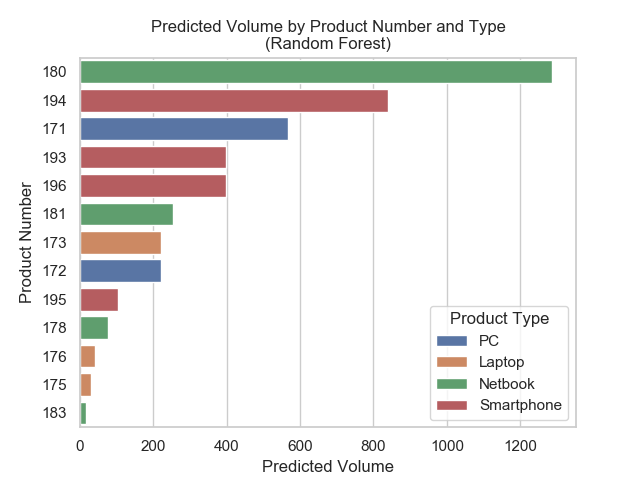
\includegraphics[width=0.75\linewidth,keepaspectratio]{predicted_volume_rf.png}
\end{figure}

\begin{figure}
    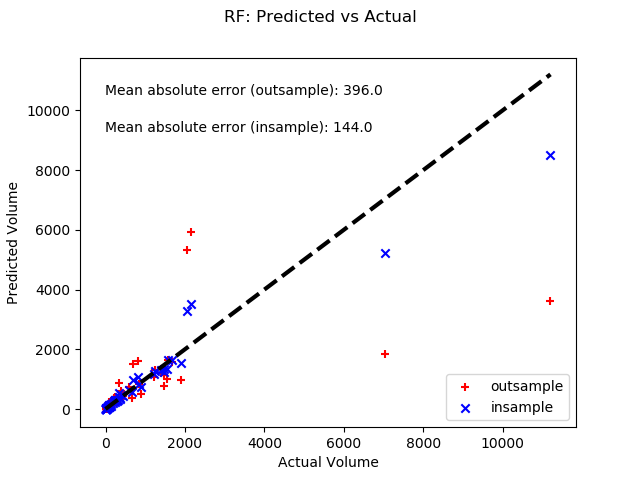
\includegraphics[width=0.75\linewidth,keepaspectratio]{predictions_final_rf.png}
\end{figure}
}

\end{columns}

\end{frame}

%------------------------------------------------
\subsection{Assessing Electronidex Sales Profile} % A subsection can be created just before a set of slides with a common theme to further break down your presentation into chunks
%------------------------------------------------

\begin{frame}
\frametitle{Assessing Electronidex Sales Profile}

\begin{columns}[c] % The "c" option specifies centered vertical alignment while the "t" option is used for top vertical alignment

\column{.4\textwidth} % Left column and width

\textbf{Problem:} Is Electronidex product line compatible to ours and are there potential
cross-selling possibilities

\uncover<2->{
\textbf{Solution:} Find product categories that are overlapping and those
that fit together and do a market basket analysis of their sales data
}

\uncover<3->{
\textbf{Knowledge Gained:} About 50 \% of our current profits come from products that overlap with
Electronidex offerings. There seems to be customer group that we do not serve at the moment and which
would be interested in our products.
}

\column{.6\textwidth} % Right column and width

\uncover<1->{
\begin{figure}
    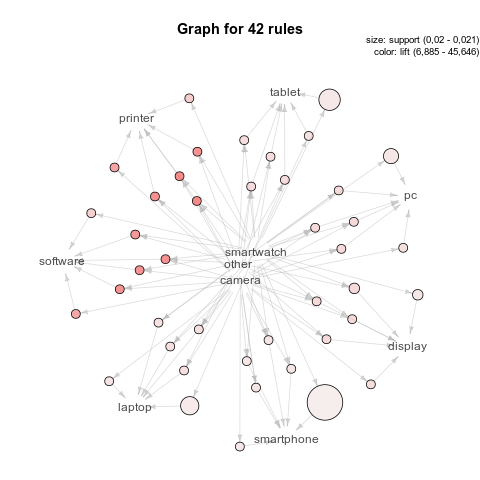
\includegraphics[width=1.0\linewidth,keepaspectratio]{apriori_product_category_level_graph.png}
\end{figure}
}

\end{columns}

\end{frame}

%------------------------------------------------
\section{Lessons Learned}
%------------------------------------------------

\begin{frame}
\frametitle{Lessons Learned}

\begin{enumerate}
    \item

        \textbf{Lesson:} Data mining can be used to help further analysis of the data by fixing its problems

    \pause
        \textbf{Advice:} Find important datasets where we have problems with data quality and try to fix this
        by creating models to correct the errors
        
    \item

    \pause
        \textbf{Lesson:} We can glean predictive information from even very small datasets, but predictive models
        created from this kind of data can only give very rough estimates

    \pause
        \textbf{Advice:} More investments in gathering high quality data from our processes and products

    \pause
    \item

    \pause
        \textbf{Lesson:} Poorly defined questions are hard to answer especially when datasets are big

    \pause
        \textbf{Advice:} Collaborate with data scientists while still at the process of formulating
        the business questions and before acquiring the data

    \pause
    \item

    \pause
        \textbf{Lesson:} Datasets can contain information whose value is not clear from the dataset itself

    \pause
        \textbf{Advice:} Pair data scientists with analysts that have relevant domain expertise

\end{enumerate}

\end{frame}

\begin{frame}
\frametitle{The End}

\Huge{\centerline{Questions?}}

\end{frame}

%----------------------------------------------------------------------------------------

\end{document}
